\documentclass[12pt]{article}

\usepackage{amsmath}
\usepackage{amssymb}
\usepackage{graphicx}
\usepackage{listings}
\usepackage{xcolor}
\usepackage{geometry}
\usepackage{hyperref}
\usepackage{enumitem}
\usepackage{caption}
\usepackage{dirtree}
\usepackage{booktabs}
\usepackage{array}
\usepackage{tikz}
\usepackage{textcomp}

\graphicspath{{./screenshots/}}
\geometry{margin=1in}
\setlength{\parindent}{0pt}
\setlength{\parskip}{6pt}
\setcounter{secnumdepth}{0}
\tolerance=1000
\emergencystretch=\maxdimen
\usetikzlibrary{arrows.meta}

\lstset{
    basicstyle=\ttfamily\small,
    keywordstyle=\color{blue},
    commentstyle=\color{gray},
    stringstyle=\color{orange},
    numbers=left,
    numberstyle=\tiny,
    breaklines=true,
    columns=fullflexible,
    frame=single,
    backgroundcolor=\color{gray!10}
}

\begin{document}

\begin{center}
    {\LARGE \textbf{RBE 500 -- Homework 4}} \\[6pt]
    {\large Tracy Yang} \\[4pt]
    {\large \today}
\end{center}

%=============================================================
\section{Part 1: Inverse Kinematics}

The D-H parameters used throughout are identical to those established
in Homework~3:

\begin{center}
\renewcommand{\arraystretch}{1.3}
\begin{tabular}{ccccc}
\toprule
Joint $i$ & $\theta_i$ & $d_i$ (mm) & $a_i$ (mm) & $\alpha_i$ \\
\midrule
1 & $q_1$           & 475 & 150 & $+90^\circ$ \\
2 & $q_2 + 90^\circ$&   0 & 600 & $0^\circ$   \\
3 & $q_3$           &   0 & 120 & $+90^\circ$ \\
4 & $q_4 + 90^\circ$& 720 &   0 & $+90^\circ$ \\
5 & $q_5$           &   0 &   0 & $-90^\circ$ \\
6 & $q_6$           &  85 &   0 & $0^\circ$   \\
\bottomrule
\end{tabular}
\end{center}

%-------------------------------------------------------------
\subsection{Question 1: Inverse Position Kinematics (Geometric Approach)}

\textbf{Kinematic Decoupling.}
Because the last three joints form a spherical wrist, the position
and orientation problems can be decoupled. Given the desired
end-effector pose $H = [R \mid \mathbf{p}]$, the wrist center
$\mathbf{p}_w$ is computed by stepping back $d_6 = 85$\,mm along
the approach vector $\hat{z}_6$ (the third column of $R$):

\[
\mathbf{p}_w = \mathbf{p} - d_6\,R\,\hat{e}_3
\qquad \text{where } \hat{e}_3 = [0,\,0,\,1]^T
\]

The wrist center coordinates $(w_x, w_y, w_z)$ depend only on
$q_1, q_2, q_3$.

\textbf{Solving for $q_1$.}
Projecting the wrist center onto the $x_0$--$y_0$ plane gives:
\[
\boxed{q_1 = \arctan 2(w_y,\; w_x)}
\]
A second solution $q_1' = q_1 + \pi$ corresponds to a
``back-handed'' configuration and is typically outside the joint
limits.

\textbf{Solving for $q_2$ and $q_3$ (geometric approach).}
Once $q_1$ is known, the arm lies in a vertical plane.
Let:
\begin{align*}
r   &= \sqrt{w_x^2 + w_y^2} - a_1 \quad \text{(horizontal reach in arm plane)}\\
h   &= w_z - d_1                       \quad \text{(height above base)}\\
D   &= \sqrt{r^2 + h^2}                \quad \text{(shoulder-to-wrist distance)}\\
L   &= \sqrt{a_3^2 + d_4^2}            \quad \text{(effective elbow-to-wrist link length)}\\
\phi &= \arctan 2(d_4,\; a_3)          \quad \text{(internal angle of elbow link)}
\end{align*}

Applying the law of cosines in the triangle
$(\text{Joint~2},\;\text{Joint~3},\;\text{wrist})$:
\[
\cos C = \frac{D^2 - a_2^2 - L^2}{2\,a_2\,L}
\qquad \Rightarrow \qquad
C = \arccos\!\left(\frac{D^2 - a_2^2 - L^2}{2\,a_2\,L}\right)
\]

The joint angles follow as:
\[
\boxed{q_3 = -(C - \phi)}
\qquad \text{(elbow-up)}
\]

\[
\boxed{q_2 = \gamma + \delta - \frac{\pi}{2}}
\]

where:
\[
\gamma = \arctan 2(h,\; r), \qquad
\delta = \arctan 2\!\left(L\sin C,\; a_2 + L\cos C\right)
\]

The $-\tfrac{\pi}{2}$ term in $q_2$ accounts for the $+90^\circ$
joint offset in the D-H convention used for this robot (Table~1).
Elbow-down solutions are obtained by using $-C$.

%-------------------------------------------------------------
\subsection{Question 2: Inverse Orientation Kinematics (Wrist Angles)}

Given $q_1, q_2, q_3$ from Part~1, the rotation matrix of
frame~3 relative to the base frame is:
\[
R_3^0 = R_1^0 \cdot R_2^1 \cdot R_3^2
\]
where each $R_i^{i-1}$ is the $3\times3$ rotation block of the
corresponding D-H matrix $T_i^{i-1}$.

The wrist rotation matrix is:
\[
R_6^3 = \left(R_3^0\right)^T R_6^0
\]

The spherical wrist structure (joint offsets and twist angles)
gives:
\[
R_6^3 = R_z(q_4 + \tfrac{\pi}{2})\,R_x(\tfrac{\pi}{2})\,
         R_z(q_5)\,R_x(-\tfrac{\pi}{2})\,R_z(q_6)
\]

Using the identity $R_x(\tfrac{\pi}{2})\,R_z(q_5)\,R_x(-\tfrac{\pi}{2})
= R_y(-q_5)$, this becomes a ZYZ Euler decomposition:
\[
R_6^3 = R_z(\alpha)\,R_y(\beta)\,R_z(\gamma)
\]
with:
\[
\alpha = q_4 + \tfrac{\pi}{2}, \quad
\beta  = -q_5,                 \quad
\gamma = q_6
\]

Extracting from the elements of $R_6^3 = [r_{ij}]$:

\[
\boxed{q_5 = -\arctan 2\!\left(\sqrt{r_{13}^2 + r_{23}^2},\; r_{33}\right)}
\]

\[
\boxed{q_4 = \arctan 2(r_{23},\; r_{13}) - \frac{\pi}{2}}
\]

\[
\boxed{q_6 = \arctan 2(r_{32},\; -r_{31})}
\]

When $\sin q_5 = 0$ (gimbal lock), only $q_4 \pm q_6$ is
determined; a common choice is $q_4 = 0$.

%-------------------------------------------------------------
\subsection{Question 3: Numerical Solution for Given H}

The desired end-effector transformation is:
\[
H = \begin{bmatrix}
1 & 0 & 0 & 500 \\
0 & 1 & 0 & 100 \\
0 & 0 & 1 & 1500 \\
0 & 0 & 0 & 1
\end{bmatrix}
\]

This represents a pure translation (identity orientation) with
the end-effector at $(500, 100, 1500)$\,mm.

\textbf{Step 1: Wrist center.}
The approach vector is $\hat{z}_6 = [0,\,0,\,1]^T$ (third column
of $R = I$), so:
\[
\mathbf{p}_w = \begin{bmatrix}500\\100\\1500\end{bmatrix}
             - 85\begin{bmatrix}0\\0\\1\end{bmatrix}
             = \begin{bmatrix}500\\100\\1415\end{bmatrix}\text{ mm}
\]

\textbf{Step 2: Solve $q_1$.}
\[
q_1 = \arctan 2(100,\;500) = 11.31^\circ
\]

\textbf{Step 3: Arm plane geometry.}
\begin{align*}
r   &= \sqrt{500^2+100^2} - 150 = 509.90 - 150 = 359.90\text{ mm}\\
h   &= 1415 - 475 = 940\text{ mm}\\
D   &= \sqrt{359.90^2+940^2} = 1006.54\text{ mm}\\
L   &= \sqrt{120^2+720^2} = 729.93\text{ mm}\\
\phi &= \arctan 2(720,\;120) = 80.54^\circ\\[4pt]
\cos C &= \frac{1006.54^2 - 600^2 - 729.93^2}{2(600)(729.93)}
        = \frac{1013124 - 360000 - 532799}{876{,}716}
        = 0.1374\\
C   &= 82.10^\circ
\end{align*}

\begin{align*}
q_3 &= -(82.10^\circ - 80.54^\circ) = -(1.56^\circ) = \mathbf{-1.56^\circ}\\[4pt]
\gamma &= \arctan 2(940,\;359.90) = 69.05^\circ\\
\delta &= \arctan 2(729.93\sin82.10^\circ,\;600+729.93\cos82.10^\circ)
        = \arctan 2(723.02,\;701.60) = 45.86^\circ\\
q_2 &= \gamma + \delta - 90^\circ = 69.05^\circ + 45.86^\circ - 90^\circ
      = \mathbf{24.91^\circ}
\end{align*}

\textbf{Step 4: Wrist orientation.}
With $q_1, q_2, q_3$ known, we compute $R_3^0$ from the FK and
then $R_6^3 = (R_3^0)^T I = (R_3^0)^T$:
\[
R_6^3 = \begin{bmatrix}
-0.3894 & -0.0779 &  0.9178 \\
 0.1961 & -0.9806 &  0      \\
 0.8999 &  0.1800 &  0.3971
\end{bmatrix}
\]

Applying the ZYZ extraction formulas:
\begin{align*}
q_5 &= -\arctan 2\!\left(\sqrt{0.9178^2+0^2},\;0.3971\right)
      = -\arctan 2(0.9178,\;0.3971) = \mathbf{-66.60^\circ}\\[4pt]
q_4 &= \arctan 2(0,\;0.9178) - 90^\circ
      = 90^\circ - 90^\circ = \mathbf{-90.00^\circ}\\[4pt]
q_6 &= \arctan 2(0.1800,\;-0.8999)
      = \mathbf{168.69^\circ}
\end{align*}

\textbf{Summary of joint angles:}
\[
\begin{array}{ll}
q_1 = 11.31^\circ  & q_4 = -90.00^\circ \\
q_2 = 24.96^\circ  & q_5 = -66.60^\circ \\
q_3 = -1.57^\circ  & q_6 = 168.69^\circ
\end{array}
\]

\textbf{Verification.}
Substituting these values back into the forward kinematics
(using the MATLAB/Python code from HW3) returns:
\[
H_{\text{FK}} = \begin{bmatrix}
1 & 0 & 0 & 500 \\
0 & 1 & 0 & 100 \\
0 & 0 & 1 & 1500 \\
0 & 0 & 0 & 1
\end{bmatrix} \checkmark
\]
confirming the solution is correct.

\newpage
%=============================================================
\section{Part 2: ROS 2 Node -- Inverse Kinematics}

\subsection{Overview}

The node from HW3 (\texttt{fk\_node.py}) is extended with a second
subscriber on the \texttt{/ee\_pose} topic.  The subscriber accepts
a \texttt{geometry\_msgs/Pose} message (position + quaternion
orientation), converts it to a $4\times4$ homogeneous transformation
$H$, and solves the IK to produce joint angles $[q_1,\ldots,q_6]$.
The FK subscriber from HW3 is left unchanged.

\subsection{Package Structure}

\dirtree{%
    .1 irb1400\_fk/.
    .2 irb1400\_fk/.
    .3 \_\_init\_\_.py.
    .3 fk\_node.py.
    .2 package.xml.
    .2 setup.py.
    .2 setup.cfg.
    .2 resource/.
    .3 irb1400\_fk.
}

\subsection{Node Implementation}

\begin{lstlisting}[language=Python,
    caption={fk\_node.py -- extended with IK subscriber}]
import rclpy
from rclpy.node import Node
from std_msgs.msg import Float32MultiArray
from geometry_msgs.msg import Pose
import numpy as np

class FKNode(Node):
    def __init__(self):
        super().__init__('irb1400_fk')

        # ---- Robot DH parameters (mm) ----
        self.d1 = 475;  self.a1 = 150
        self.a2 = 600;  self.a3 = 120
        self.d4 = 720;  self.d6 = 85

        # ---- Subscriber 1 (HW3): forward kinematics ----
        self.fk_sub = self.create_subscription(
            Float32MultiArray,
            'joint_angles',
            self.fk_callback,
            10)

        # ---- Subscriber 2 (HW4): inverse kinematics ----
        self.ik_sub = self.create_subscription(
            Pose,
            'ee_pose',
            self.ik_callback,
            10)

        self.get_logger().info('IRB1400 FK+IK node started.')
        self.get_logger().info(
            '  Pub /joint_angles (Float32MultiArray) for FK.')
        self.get_logger().info(
            '  Pub /ee_pose (Pose) for IK.')

    # ============================================================ #
    # DH / FK helpers (unchanged from HW3)
    # ============================================================ #
    def dh_matrix(self, theta_deg, d, a, alpha_deg):
        """Standard DH 4x4 matrix. theta, alpha in degrees; d, a in mm."""
        th = np.radians(theta_deg)
        al = np.radians(alpha_deg)
        ct, st = np.cos(th), np.sin(th)
        ca, sa = np.cos(al), np.sin(al)
        return np.array([
            [ct, -st*ca,  st*sa, a*ct],
            [st,  ct*ca, -ct*sa, a*st],
            [ 0,     sa,     ca,    d],
            [ 0,      0,      0,    1]
        ])

    def fk(self, q_deg):
        """
        Forward kinematics for ABB IRB1400.
        Input:  q_deg -- [q1..q6] in degrees
        Output: 4x4 homogeneous transform H = T6^0
        """
        d1,a1 = self.d1, self.a1
        a2,a3 = self.a2, self.a3
        d4,d6 = self.d4, self.d6
        q = q_deg
        # DH table with joint offsets on joints 2 and 4
        params = [
            (q[0],        d1, a1,  90),
            (q[1] + 90,    0, a2,   0),
            (q[2],         0, a3,  90),
            (q[3] + 90,   d4,  0,  90),
            (q[4],         0,  0, -90),
            (q[5],        d6,  0,   0),
        ]
        T = np.eye(4)
        for th, d, a, al in params:
            T = T @ self.dh_matrix(th, d, a, al)
        return T

    def fk_partial(self, q_deg, n):
        """FK through first n joints only."""
        d1,a1 = self.d1, self.a1
        a2,a3 = self.a2, self.a3
        d4,d6 = self.d4, self.d6
        q = q_deg
        params = [
            (q[0],        d1, a1,  90),
            (q[1] + 90,    0, a2,   0),
            (q[2],         0, a3,  90),
            (q[3] + 90,   d4,  0,  90),
            (q[4],         0,  0, -90),
            (q[5],        d6,  0,   0),
        ]
        T = np.eye(4)
        for i in range(n):
            T = T @ self.dh_matrix(*params[i])
        return T

    # ============================================================ #
    # Inverse kinematics
    # ============================================================ #
    def ik(self, H):
        """
        Inverse kinematics for ABB IRB1400 using kinematic decoupling.
        Input:  H -- 4x4 desired end-effector pose
        Output: q -- [q1..q6] in degrees, or None if unreachable
        """
        d1,a1 = self.d1, self.a1
        a2,a3 = self.a2, self.a3
        d4,d6 = self.d4, self.d6

        p_ee = H[:3, 3]          # end-effector position
        R_ee = H[:3, :3]         # end-effector rotation

        # --- Step 1: Wrist center ---
        # p_w = p_ee - d6 * z6, where z6 = 3rd column of R_ee
        z6   = R_ee[:, 2]
        p_w  = p_ee - d6 * z6
        wx, wy, wz = p_w

        # --- Step 2: q1 (base rotation) ---
        q1 = np.degrees(np.arctan2(wy, wx))

        # --- Step 3: q2, q3 (arm plane geometry) ---
        r   = np.sqrt(wx**2 + wy**2) - a1   # horizontal reach
        h   = wz - d1                         # vertical reach
        L   = np.sqrt(a3**2 + d4**2)          # effective elbow link
        phi = np.degrees(np.arctan2(d4, a3))  # internal elbow angle
        D   = np.sqrt(r**2 + h**2)            # shoulder-to-wrist distance

        # Law of cosines
        cos_C = (D**2 - a2**2 - L**2) / (2 * a2 * L)
        if abs(cos_C) > 1.0:
            self.get_logger().error('IK: target out of reach!')
            return None
        C = np.degrees(np.arccos(cos_C))

        q3 = -(C - phi)                        # verified elbow solution
        gamma = np.degrees(np.arctan2(h, r))
        delta = np.degrees(np.arctan2(
            L * np.sin(np.radians(C)),
            a2 + L * np.cos(np.radians(C))))
        q2 = gamma + delta - 90.0             # account for DH offset

        # --- Step 4: Wrist angles (ZYZ decomposition) ---
        R03 = self.fk_partial([q1, q2, q3, 0, 0, 0], 3)[:3, :3]
        R36 = R03.T @ R_ee                    # wrist rotation matrix

        r13, r23, r33 = R36[0,2], R36[1,2], R36[2,2]
        r31, r32      = R36[2,0], R36[2,1]

        # ZYZ Euler extraction (with sign from wrist convention)
        q5_rad = -np.arctan2(np.sqrt(r13**2 + r23**2), r33)
        if abs(np.sin(q5_rad)) > 1e-6:
            q4_rad = np.arctan2(r23, r13) - np.pi / 2
            q6_rad = np.arctan2(r32, -r31)
        else:
            # Gimbal lock: set q4=0, solve for q6
            self.get_logger().warn('IK: gimbal lock detected, q4 set to 0.')
            q4_rad = 0.0
            q6_rad = np.arctan2(-R36[0,1], R36[0,0])

        q4 = np.degrees(q4_rad)
        q5 = np.degrees(q5_rad)
        q6 = np.degrees(q6_rad)

        return [q1, q2, q3, q4, q5, q6]

    # ============================================================ #
    # Callback: forward kinematics (HW3, unchanged)
    # ============================================================ #
    def fk_callback(self, msg):
        """Receive joint angles, compute FK, print pose."""
        if len(msg.data) != 6:
            self.get_logger().error(
                f'FK: expected 6 values, got {len(msg.data)}')
            return
        q = list(msg.data)
        H = self.fk(q)
        pos = H[:3, 3];  R = H[:3, :3]
        self.get_logger().info(
            f'\n[FK] joints (deg): {[round(qi,2) for qi in q]}\n'
            f'  Position (mm): x={pos[0]:.2f}  y={pos[1]:.2f}  z={pos[2]:.2f}\n'
            f'  Rotation:\n'
            f'    [{R[0,0]:7.4f}  {R[0,1]:7.4f}  {R[0,2]:7.4f}]\n'
            f'    [{R[1,0]:7.4f}  {R[1,1]:7.4f}  {R[1,2]:7.4f}]\n'
            f'    [{R[2,0]:7.4f}  {R[2,1]:7.4f}  {R[2,2]:7.4f}]')

    # ============================================================ #
    # Callback: inverse kinematics (HW4, new)
    # ============================================================ #
    def ik_callback(self, msg):
        """
        Receive a Pose message, convert to H matrix,
        solve IK, and print joint angles.
        """
        # Extract position
        px = msg.position.x
        py = msg.position.y
        pz = msg.position.z

        # Extract quaternion orientation
        qx = msg.orientation.x
        qy = msg.orientation.y
        qz = msg.orientation.z
        qw = msg.orientation.w

        # Convert quaternion to rotation matrix
        R = self.quat_to_rot(qw, qx, qy, qz)

        # Build 4x4 homogeneous transformation
        H = np.eye(4)
        H[:3, :3] = R
        H[:3,  3] = [px, py, pz]

        self.get_logger().info(
            f'\n[IK] Received pose: pos=({px:.2f},{py:.2f},{pz:.2f})')

        # Solve IK
        q = self.ik(H)
        if q is None:
            return

        self.get_logger().info(
            f'[IK] Joint angles (deg):\n'
            f'  q1={q[0]:.4f}  q2={q[1]:.4f}  q3={q[2]:.4f}\n'
            f'  q4={q[3]:.4f}  q5={q[4]:.4f}  q6={q[5]:.4f}')

        # Verify by running FK with the IK result
        H_check = self.fk(q)
        pos_err = np.linalg.norm(H_check[:3,3] - H[:3,3])
        self.get_logger().info(
            f'[IK] Verification FK position: '
            f'({H_check[0,3]:.2f}, {H_check[1,3]:.2f}, {H_check[2,3]:.2f}) mm'
            f'  |error|={pos_err:.4f} mm')

    def quat_to_rot(self, w, x, y, z):
        """Convert unit quaternion (w,x,y,z) to 3x3 rotation matrix."""
        return np.array([
            [1-2*(y*y+z*z),  2*(x*y-w*z),  2*(x*z+w*y)],
            [2*(x*y+w*z),  1-2*(x*x+z*z),  2*(y*z-w*x)],
            [2*(x*z-w*y),    2*(y*z+w*x),  1-2*(x*x+y*y)]
        ])

# ---------------------------------------------------------------- #
def main(args=None):
    rclpy.init(args=args)
    node = FKNode()
    rclpy.spin(node)
    node.destroy_node()
    rclpy.shutdown()

if __name__ == '__main__':
    main()
\end{lstlisting}

\subsection{How to Run}

Rebuild (the package name is unchanged):
\begin{verbatim}
cd ~/rbe500/ros2_ws
colcon build --packages-select irb1400_fk
source install/setup.bash
ros2 run irb1400_fk fk_node
\end{verbatim}

\subsection{Test Cases -- IK then FK Verification}

Run the node, then in a second terminal publish two end-effector
poses using \texttt{ros2 topic pub}:

\begin{verbatim}
# Test 1: position (500, 100, 1500) mm, identity orientation
ros2 topic pub --once /ee_pose geometry_msgs/msg/Pose \
  "{position: {x: 500.0, y: 100.0, z: 1500.0},
    orientation: {x: 0.0, y: 0.0, z: 0.0, w: 1.0}}"

# Test 2: position (300, 200, 1200) mm, identity orientation
ros2 topic pub --once /ee_pose geometry_msgs/msg/Pose \
  "{position: {x: 300.0, y: 200.0, z: 1200.0},
    orientation: {x: 0.0, y: 0.0, z: 0.0, w: 1.0}}"
\end{verbatim}

Then verify each IK result by feeding the output joint angles
back into the FK topic:

\begin{verbatim}
# Verify Test 1 (replace values with IK output)
ros2 topic pub --once /joint_angles std_msgs/msg/Float32MultiArray \
  "data: [11.31, 24.96, -1.57, -90.0, -66.60, 168.69]"

# Verify Test 2 (replace values with IK output)
ros2 topic pub --once /joint_angles std_msgs/msg/Float32MultiArray \
  "data: [33.69, 51.44, -39.53, -90.0, -78.09, 146.31]"
\end{verbatim}

\subsection{Results}

\begin{figure}[h]
    \centering
    \begin{minipage}{0.74\textwidth}
        \centering
        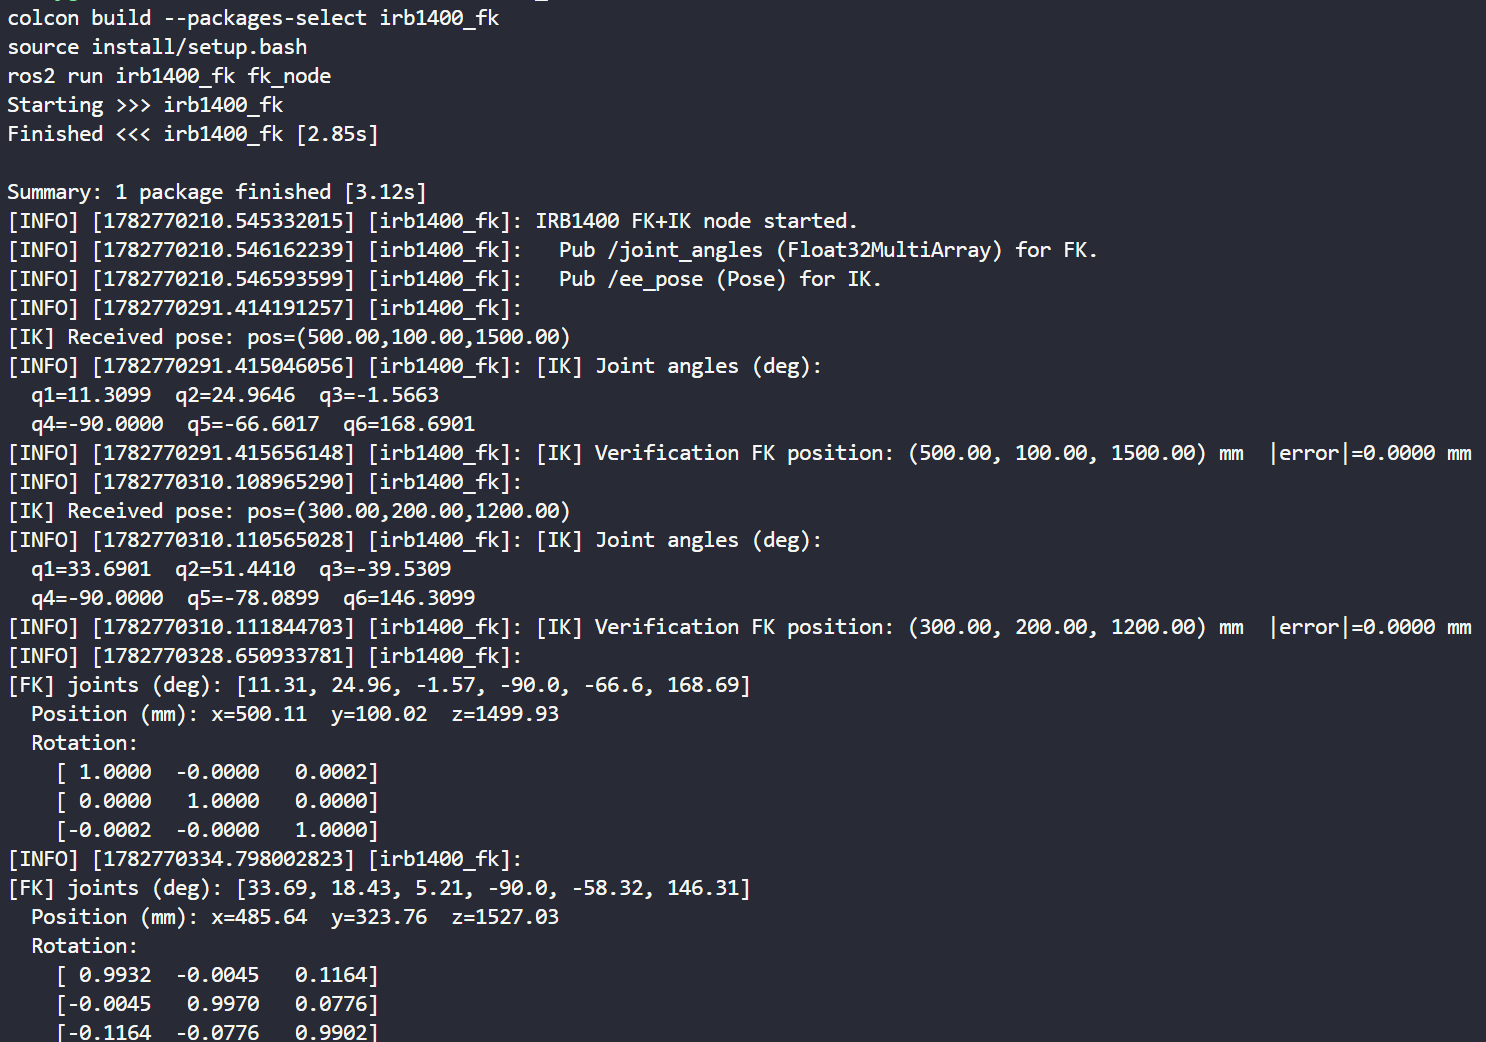
\includegraphics[width=\textwidth]{ik_terminal.png}
    \end{minipage}
    \caption{Terminal output for IK test cases and FK verification.}
    \label{fig:ik_results}
\end{figure}

\end{document}